\chapter{Literature Review}
In today’s competitive landscape, modern transcription-based applications and meeting asssistants increasingly integrate chat-based interfaces to allow users to query recorded conversations. In approaching the development of this project, a comprehensive review was conducted on the retrieval capabilities of three existing products: Otter.ai, Claude Code and the existing Meadow9+ mobile application. These products were selected due to their relevance to the proposed project. 

The literature review focused on three key aspects: retrieval strategies, accuracy and latency characteristics, and transparency of retrieval and reasoning. Instead of trying to replicate existing solutions, this review aimed to understand how these platforms effectively address retrieval challenges and identify opportunities for improvement in developing our project. An in-depth analysis of the technological stacks and architectures will be presented in later chapters, specifically in the context of Meadow9+, as such information is not publicly available for the other products reviewed.

This chapter is divided into three main sections. Section 2.1 reviews Otter.ai, and Section 2.2 examines Claude Code, focusing exclusively on their retrieval system. Section 2.3 evaluates the Meadow9+ mobile application prior to this project. 

\section{Otter.ai}
Otter.ai is a widely adopted speech-to-text and meeting assistant platform that provides real-time transcription, post-meeting summaries, and multiple mechanisms for retrieving information from recorded conversations \cite{otter_appstore}. As a mature commercial system, it represents a strong baseline for evaluating existing approaches to transcript retrieval and conversational interaction. 

Otter.ai caters to a wide range of users, including businesses and students \cite{otter_sales_agent,otter_education_agent}. While it is primarily used for transcribing meetings, the platform also proves valuable for sales calls and lecture notes \cite{otter_sales_agent,otter_education_agent}. While Otter.ai offers applications on different platforms including web, iOS and Android \cite{otter_features}, this discussion will focus exclusively on the iOS application.

\subsection{Retrieval Strategies}
Otter.ai provides three primary mechanisms for retrieving information from transcripts: keyword-based search, LLM-powered conversational querying (Otter AI Chat), and LLM-Based Summarization, as illustrated in Figure \ref{fig:otter-interface} \cite{otter_appstore,otter_features}.

\begin{figure}[H]
  \centering
  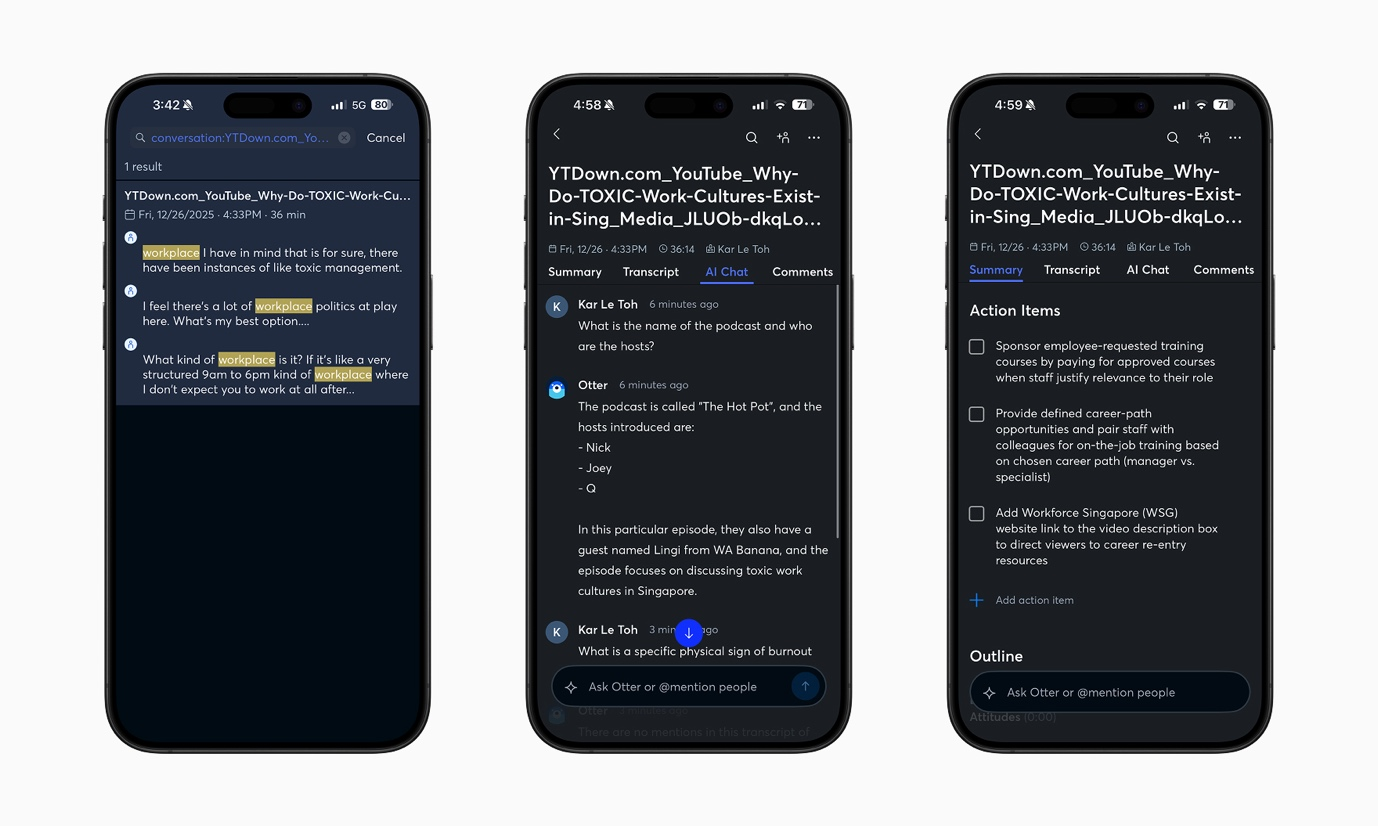
\includegraphics[width=1.0\textwidth]{figures/otter_ai_ios_application_interface_showing_keyword_search_ai_chat_and_summarization_features.jpeg}
  \caption{Otter.ai iOS application interface showing keyword search, AI chat, and summarization features}
  \label{fig:otter-interface}
\end{figure}

Keyword-Based Retrieval

Otter.ai supports keyword-based search over notes and transcripts \cite{otter_features}. Although Otter.ai does not publicly disclose the exact retrieval algorithm used, empirical testing suggests that the system employs a term-weighted ranking function such as TF-IDF or BM25. For example, queries containing additional discriminative terms such as “toxic workplace” versus “workplace” significantly alter result rankings in a manner consistent with BM25-style term frequency saturation and inverse document frequency weighting \cite{robertson2009bm25}. In addition, Otter.ai supports date-based filters over transcript metadata \cite{otter_features}. This feature substantially improves usability and demonstrates the value of combining structured metadata filtering with unstructured text search.

LLM-Based Conversational Retrieval (Otter AI Chat)

Otter AI Chat allows users to ask free-form natural language questions either across all transcripts or within a specific transcript. While Otter.ai does not explicitly disclose its backend architecture, its FAQ indicates that transcript content and prompts are transmitted to third-party services only when users actively interact with Otter AI Chat, strongly suggesting reliance on externally hosted LLMs from third-party providers \cite{otter_ai_chat_faq}.

Behavioral observations indicate that the global chat interface likely employs a retrieval step to narrow down relevant transcripts before passing context to the LLM, as responses often include links to specific conversations. This behavior is consistent with a RAG pipeline operating at the document level. In contrast, the per-transcript chat interface appears to process the entire transcript holistically, as responses rarely reference precise supporting segments or timestamps.

Notably, Otter AI Chat responses tend to be abstractive and conversational, favoring rephrased summaries over verbatim quotations. This design choice may be driven by prompt engineering rather than retrieval limitations; however, it also suggests limited emphasis on fine-grained, chunk-level semantic retrieval at query time. 

LLM-Based Summarization

Beyond interactive retrieval, Otter.ai generates an extensive per-transcript summary using LLM-based processing \cite{otter_appstore}. This summary is structured into three layers: (i) a high-level overview of the meeting, (ii) extracted action items, and (iii) a hierarchical outline organized by timestamps, with further speaker-segmented summaries nested within each time interval. This multi-level summarization demonstrates effective use of LLMs to transform long-form transcripts into structured, navigable representations. 

\subsection{Accuracy and Latency Characteristics}
From manual evaluation, Otter.ai’s keyword-based search exhibits both high accuracy and negligible latency, consistent with expectations for traditional lexical retrieval systems. This makes keyword search the most reliable and responsive mechanism for precise information lookup. Otter AI Chat, when applied to transcripts up to approximately two hours in length, also demonstrates low perceived latency and strong answer accuracy. This performance is likely enabled by the use of large, cloud-hosted LLMs with sufficient context windows and optimized inference infrastructure.

\subsection{Transparency of Retrieval and Reasoning}
A notable limitation of Otter AI Chat is its lack of transparency. The system provides minimal visibility into which transcript segments support a given answer, and users cannot inspect or verify the retrieved evidence. This opacity limits user trust and makes error diagnosis difficult, particularly in professional or compliance-sensitive settings.

\subsection{Discussion and Implications}
Overall, Otter.ai exemplifies a feature-rich and well-integrated retrieval ecosystem for meeting transcripts. It combines global and local keyword search, conversational querying, and comprehensive summarization to support diverse user workflows. These capabilities collectively demonstrate that effective transcript systems must treat retrieval as a first-class design concern, rather than a secondary feature layered on top of transcription.

However, the apparent lack of fine-grained, chunk-level grounding and the absence of explicit evidence attribution indicate that Otter.ai’s system prioritizes fluency and abstraction over verifiability. While this design choice may be acceptable for general meeting summarization, it introduces risks of hallucination and reduces user trust in scenarios where factual accuracy and traceability are critical. This limitation is particularly relevant to Meadow9+, since it cannot rely on large cloud-hosted frontier models with extensive context windows and optimized inference pipelines. Instead, it employs a smaller, self-hosted LLM with stricter latency and context constraints. Consequently, passing full transcripts, or even large document-level contexts, into the model is neither scalable nor reliable.

These observations collectively imply that Meadow9+ must adopt a \textit{more retrieval-centric and evidence-grounded design} than Otter.ai. Rather than treating retrieval as a preliminary filtering step, retrieval must be a first-class system component that operates at multiple granularities (document-level, chunk-level, and temporal level). Figure 2.1 illustrates the baseline chatbot architecture commonly observed in existing systems, where retrieval is shallow or opaque and tightly coupled to generation.

In contrast, Meadow9+ is designed to decouple retrieval from generation and to emphasize transparent, inspectable retrieval results. This includes (i) hybrid lexical--semantic retrieval to handle both exact terms and paraphrased queries, (ii) phonetic and fuzzy matching to mitigate transcription errors, and (iii) chunk-level evidence selection to reduce prompt length. By explicitly surfacing retrieved segments and their timestamps, Meadow9+ aims to improve both answer accuracy and user trust, which is an aspect largely absent in Otter.ai’s conversational interface.

\section{Claude Code}
Recent advances in LLM--based agents have extended beyond conversational assistants into domain-specialized systems that tightly integrate retrieval, reasoning, and action. One notable example is Claude Code, a command-line interface (CLI) agent developed by Anthropic that brings LLM-driven reasoning directly into the software development workflow \cite{anthropic_claude_code_tutorials}. Claude Code is widely regarded as one of the most capable coding agents currently available, not solely due to model quality, but because of its system-level retrieval and context management design that enables effective reasoning over large, evolving codebases.

\subsection{Retrieval Strategies}
Claude Code adopts an agentic retrieval paradigm, where the LLM actively searches and retrieves relevant context from the environment at query time rather than relying on a precomputed embedding index or static vector store. Specifically, Claude Code is granted controlled read access to the local project directory and retrieves information by invoking standard developer tools such as file search and content matching when needed \cite{anthropic_claude_code_settings,anthropic_claude_code_team}. Retrieved files or code snippets are then injected directly into the model’s context window.

Importantly, retrieval is performed dynamically through tool calls that operate over the source-of-truth codebase rather than through a precomputed embedding index \cite{anthropic_claude_code_settings,anthropic_claude_code_team}. This design avoids issues associated with stale embeddings, incomplete indexing, and semantic drift, ensuring that the retrieved context always reflects the most recent state of the project.

Claude Code also supports persistent project-level memory via a lightweight mechanism: a configuration file (e.g., CLAUDE.md) that stores high-level instructions, architectural conventions, and recurring commands. This file is automatically injected into every session, acting as a form of long-term context without requiring a separate memory model or database \cite{anthropic_claude_code_memory}.

\subsection{Accuracy and Latency Characteristics}
The agentic retrieval strategy in Claude Code introduces clear trade-offs between accuracy and latency. On the one hand, dynamically searching the codebase yields high retrieval precision, as the agent can iteratively refine its search queries and inspect exact source files relevant to the task \cite{anthropic_claude_code_settings}. This approach can improve task success rates in complex, multi-file coding scenarios compared to static retrieval pipelines.

On the other hand, retrieval incurs non-trivial overhead. Each file read and search operation increases prompt size and introduces runtime latency due to tool execution and additional token processing. This design typically leads to higher token usage and slower individual responses compared to systems that rely on pre-indexed embeddings, but the overhead can be acceptable given the resulting improvement in task accuracy and robustness.

To further improve accuracy on complex tasks, Claude supports an extended thinking mode in which the model spends more time deliberating before producing an answer \cite{anthropic_extended_thinking}. While this increases latency, it can improve solution quality for tasks requiring multi-step reasoning or global code understanding.

\subsection{Transparency of Retrieval and Reasoning}
A defining characteristic of Claude Code is its emphasis on transparent retrieval and execution. Tool use is permission-gated, and any action that may modify the system requires user approval \cite{anthropic_claude_code_settings,anthropic_claude_code_team}. This design allows developers to observe how context is retrieved and to intervene when necessary.

Claude Code also provides a “Plan Mode,” in which the agent analyzes the codebase and proposes a sequence of actions without executing them. This separation of planning and execution improves trust and enables users to validate the agent’s understanding before committing changes \cite{anthropic_claude_code_tutorials}.

From a system-design perspective, Claude Code demonstrates that retrieval transparency is not only a safety feature but also a debugging aid, allowing users to reason about failures in retrieval or context selection.

\subsection{Discussion and Implications}
Although Claude Code operates in the domain of software engineering, its retrieval design offers several transferable insights for transcript-based systems such as Meadow9+.

First, Claude Code’s avoidance of static embedding-based retrieval highlights a broader design principle: retrieval systems must align with the nature of the underlying data. Claude Code adopts a fully agentic retrieval approach precisely because of the characteristics of its target domain. Dynamic, query-time search over the source-of-truth codebase ensures that retrieved context remains up-to-date and semantically precise, avoiding issues associated with stale or incomplete indices.

In contrast, Meadow9+ operates over transcript data that is static once transcription is completed. While a full agentic retrieval paradigm is powerful, it is not strictly required in this setting. Additionally, practical system constraints must also be considered, as Meadow9+ employs a smaller self-hosted LLM with substantially weaker reasoning and tool-use capabilities compared to commercial frontier models used in systems such as Claude Code. Under these constraints, fully agentic retrieval may introduce performance bottlenecks, increased latency, or even unstable retrieval behavior, particularly when iterative reasoning and tool invocation are required.

These observations suggest that the optimal retrieval strategy for Meadow9+ lies in a hybrid approach, combining embedding-based semantic retrieval with symbolic techniques. Such a design leverages the static nature of transcript data to enable efficient indexing while remaining robust to transcription noise and lexical variation. At the same time, it avoids the computational and reasoning overheads associated with fully agentic retrieval, making it more suitable for deployment with resource-constrained, self-hosted LLMs.

Second, Claude Code’s trade-off between accuracy and latency offers guidance for Meadow9+’s system design. Claude Code deliberately trades off latency and token efficiency in exchange for higher task accuracy. Each retrieval step incurs additional overhead due to tool invocation, file inspection, and prompt expansion. This trade-off is acceptable in developer workflows, where correctness is often prioritized over response time and where commercial frontier models with strong reasoning capabilities are available.

Meadow9+, however, operates under stricter latency and cost constraints. The system also relies on a self-hosted, smaller-scale LLM, which is significantly less capable than proprietary frontier models. Under such constraints, a fully agentic retrieval loop may introduce excessive latency and unstable performance. Moreover, iterative retrieval decisions place additional reasoning burden on the model itself, increasing the risk of suboptimal search strategies and error propagation.

These observations suggest that the retrieval strategy for Meadow9+ should be front-loaded into deterministic or weakly learned components, such as BM25 and dense embeddings, rather than delegated to the LLM. This reduces the reasoning load on the model and yields more predictable latency characteristics.

Finally, Claude Code’s emphasis on transparent retrieval suggests an additional opportunity for Meadow9+. While Meadow9+ targets non-technical users, partial transparency, such as highlighting which transcript segments were used to generate an answer, can improve user trust and perceived reliability. This is especially important in professional meeting contexts where incorrect attribution or hallucinated decisions can have serious consequences.

Incorporating lightweight transparency mechanisms aligns with Claude Code’s philosophy that retrieval visibility is not merely a safety feature but a debugging and validation aid. Such features can also support iterative refinement of retrieval strategies during system evaluation.

\section{Pre-Project Meadow9+}
Meadow9+ is a mobile speech-to-text application developed by researchers from the NTU Speech and Language Laboratory, with initial development dating back to approximately 2021 (exact date to be confirmed) \cite{meadow9_appstore_au,abax_ai_site}. It is a product of ABAX AI, a company specializing in advanced speech recognition technologies tailored for enterprise and professional use cases \cite{abax_ai_site,abax_ai_companies_sg}.

The platform is primarily designed for Singapore-based business professionals, with a strong emphasis on one-to-one meetings as its core usage scenario \cite{meadow9_appstore_au,abax_ai_site,abax_ai_companies_sg}. Nevertheless, Meadow9+ also supports a broader range of transcription contexts, including multi-party discussions and news audio recordings. A key strength of the system lies in its ability to handle Singaporean accents and domain-specific terminology, addressing a notable gap in the local speech recognition market where generic transcription systems often underperform.

While Meadow9+ demonstrates strong transcription quality, particularly in localized linguistic contexts, its post-transcription information retrieval and interaction capabilities remain limited. The following subsections analyze the retrieval and summarization mechanisms implemented in the pre-project version of Meadow9+, highlighting their strengths and limitations.

\subsection{Retrieval Strategies}
Meadow9+ provides two primary mechanisms for retrieving information from transcripts: (1) text-matching search and (2) LLM-based conversational querying.

Text-Matching Search

The system supports a text-matching search functionality at the global level, allowing users to search across conversation titles. At query time, the search matches user-provided keywords against stored conversation titles, returning transcripts whose metadata contains the queried terms. This design emphasizes simplicity and responsiveness, making it suitable for lightweight retrieval scenarios where meaningful titles are consistently available.

LLM-Based Conversational Retrieval

Meadow9+ integrates an LLM-powered chatbot that allows users to pose free-form natural language questions within a selected transcript \cite{meadow9_appstore_us}. For privacy and data governance considerations, the chatbot relies on a self-hosted LLM. 

In the pre-project system, the chatbot passes the full transcript directly into the LLM as input context at query time, without an intermediate retrieval or context selection stage. Responses generated by the system are primarily abstractive and conversational in nature, focusing on synthesized summaries rather than direct quotations or fine-grained references to specific transcript segments.

LLM-Based Summarization

In addition to interactive querying, Meadow9+ generates a per-transcript summary using LLM-based processing \cite{meadow9_appstore_us}. This summary provides a condensed overview of the meeting content and is generated independently of user queries. The summarization output is static and intended for post-meeting review rather than targeted information retrieval. It does not support interaction, filtering, or alignment with subsequent user questions.

\subsection{Accuracy and Latency Characteristics}
Based on manual evaluation, Meadow9+’s text-matching search demonstrates high accuracy and minimal latency under ideal conditions. When relevant metadata is present, search results are returned promptly.

In contrast, the chatbot exhibits high perceived latency and weak answer accuracy when applied to transcripts exceeding approximately 1 hour in length. These performance issues are likely attributable to two factors: (1) the use of a relatively small self-hosted LLM with limited reasoning capacity compared to commercial frontier models, and (2) inefficient utilization of the model’s context window due to the absence of retrieval or context selection mechanisms.

\subsection{Transparency of Retrieval and Reasoning}
The pre-project Meadow9+ chatbot presents users with a single generated response per query. The system does not provide explicit indicators of which transcript segments were most relevant to the answer, nor does it surface supporting excerpts or references from the transcript. As a result, users interact with the chatbot as a black-box conversational interface, without visibility into intermediate reasoning or evidence selection processes.

\subsection{Discussion and Implications}
The pre-project Meadow9+ system demonstrates a clear separation between transcription quality and post-transcription interaction capabilities. While the platform is optimized for accurate speech recognition in localized contexts, its retrieval and interaction mechanisms are comparatively lightweight and monolithic, exhibiting several structural limitations that impact effectiveness, scalability, and user experience.

For text-matching search, the reliance on transcript-level metadata significantly constrains retrieval coverage. Because conversation titles and descriptions are optional, many transcripts lack sufficiently descriptive metadata, reducing the practical utility of this search mechanism. Moreover, the absence of keyword-based searching within transcript content prevents users from retrieving specific terms, entities, or discussion points embedded in the conversation itself. The system also does not support natural language or temporal constraints (e.g., “last Friday” or “earlier in the meeting”), which are increasingly expected in modern retrieval interfaces.

The LLM-based conversational retrieval approach addresses some expressiveness limitations by allowing free-form queries; however, its design introduces different trade-offs. Passing entire transcripts directly to the LLM leads to high inference latency for long-duration meetings and exacerbates the lost-in-the-middle problem. Additionally, the abstractive nature of responses, combined with the lack of explicit evidence grounding, reduces answer verifiability and makes systematic error analysis difficult.

Collectively, these observations highlight a fundamental architectural gap in the pre-project Meadow9+ system: the absence of an explicit, fine-grained retrieval layer that mediates between raw transcripts and language model generation. This gap motivates the adoption of a structured RAG framework in the proposed system. By decoupling retrieval from generation and incorporating hybrid retrieval strategies tailored to noisy speech-to-text data, the redesigned system aims to improve latency, accuracy, transparency, and scalability while preserving conversational usability.
